\ifpdf

    \vspace{1cm}
    \begin{figure}[H]
        \centering
        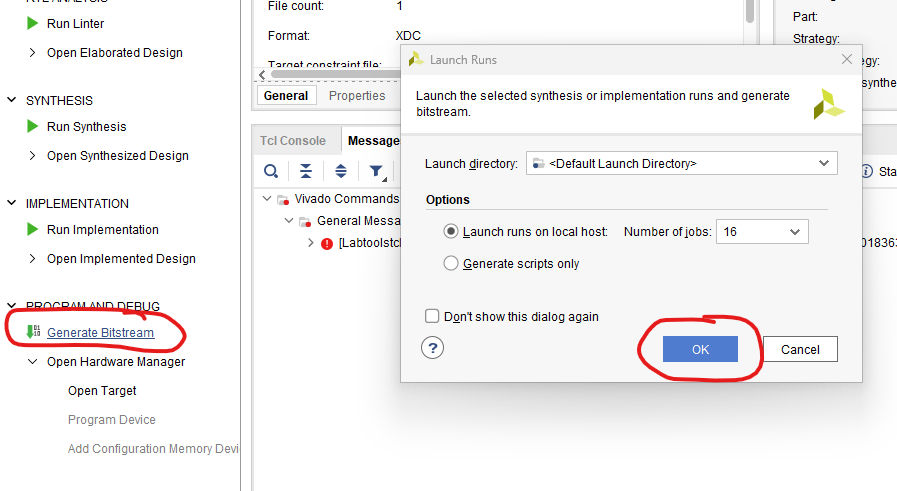
\includegraphics[width=9cm]{Images/CreateBitstreamImages/Vivado_GenerateBitstream.png}
        \caption{Click on Generate Bitstream}
        \label{fig:enter-label}
        \raggedright
        \vspace{0.5cm}
        When creating your own files you will need to simulate each file before attempting to upload it to the board. In this particular case we have validated the provided files to ensure that they work on the Basys 3 boards, so you could have clicked directly on "Generate\_Bitstream" without stepping through synthesis and implementation independently. Assuming your design sources and constraints are correctly set it should begin generating a bitstream file for the Basys 3. You can increase the number of jobs to save some time. 

    \end{figure}

    \begin{figure}[H]
        \centering
        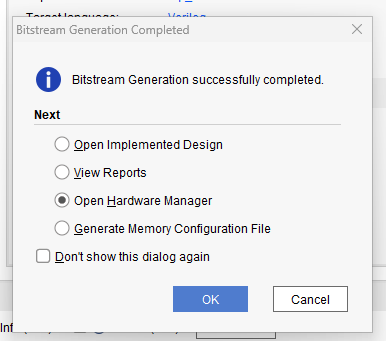
\includegraphics[width=9cm]{Images/CreateBitstreamImages/Vivado_BitstreamGenerated.png}
        \caption{Select Open Hardware Manager}
        \label{fig:enter-label}
    \end{figure}
    Once the bitstream is completed a box will pop up. Ensure that open hardware manager is selected, then hit okay.

    \begin{figure}[H]
        \centering
        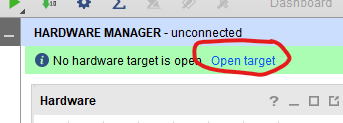
\includegraphics[width=9cm]{Images/CreateBitstreamImages/Vivado_OpenTarget.png}
        \caption{Select Open Target and hit Auto Connect}
        \label{fig:enter-label}
    \end{figure}
    This will begin the connection to the the local hardware server which Xilinx uses to talk with the Basys 3 board. If you were using a remote board then you will need to set the server IP. 
    
    \begin{figure}[H]
        \centering
        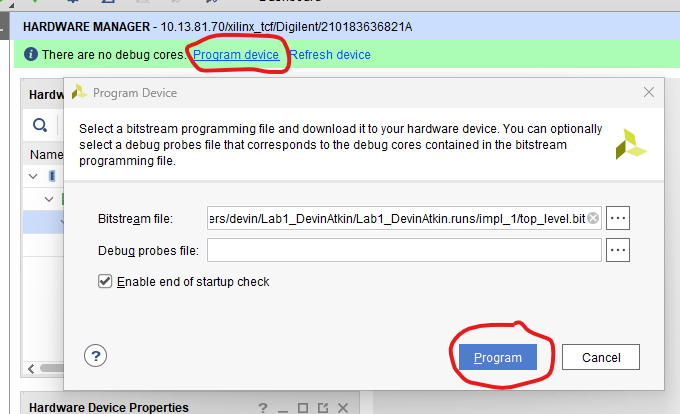
\includegraphics[width=9cm]{Images/CreateBitstreamImages/Vivado_ProgramHardware.png}
        \caption{Select Program Device}
        \label{fig:enter-label}
    \end{figure}
    Once connected you should select program device and then hit program. This should send the generated bitstream to the Xilinx hardware. Assuming no errors come up, then you should be able to tell if the programming worked by Green done LED turning on. 
\else
    \HCode{<video width="320" height="240" controls>
    <source src="Images/CreateProject_Vivado2023.mp4" type="video/mp4">
    <img src="Images/Vivado_CreateProject.png" alt="Video Shows the button press for the create project">
    Your browser does not support the video tag. (Still need to update this to a new video)
    </video>}
\fi